\documentclass[10pt,twocolumn,letterpaper]{article}

\usepackage{cvpr}
\usepackage{times}
\usepackage{epsfig}
\usepackage{graphicx}
\usepackage{amsmath}
\usepackage{amssymb}
\usepackage{float}
\usepackage{listings}
\usepackage{color} %red, green, blue, yellow, cyan, magenta, black, white
\definecolor{mygreen}{RGB}{28,172,0} % color values Red, Green, Blue
\definecolor{mylilas}{RGB}{170,55,241}
\usepackage{blindtext}

% Include other packages here, before hyperref.

% If you comment hyperref and then uncomment it, you should delete
% egpaper.aux before re-running latex.  (Or just hit 'q' on the first latex
% run, let it finish, and you should be clear).
\usepackage[breaklinks=true,bookmarks=false]{hyperref}

\cvprfinalcopy % *** Uncomment this line for the final submission

\def\cvprPaperID{****} % *** Enter the CVPR Paper ID here
\def\httilde{\mbox{\tt\raisebox{-.5ex}{\symbol{126}}}}

% Pages are numbered in submission mode, and unnumbered in camera-ready
%\ifcvprfinal\pagestyle{empty}\fi
\setcounter{page}{1}
\begin{document}

%%%%%%%%% TITLE
\title{Machine Learining for Computer Vision Coursework 1\\
	Face Recognition by PCA
	}

\author{David Angelov\\
MEng Electrical and Electronic Engineering \\
Imperial College London\\
{\tt\small david.angelov12@imperial.ac.uk}
% For a paper whose authors are all at the same institution,
% omit the following lines up until the closing ``}''.
% Additional authors and addresses can be added with ``\and'',
% just like the second author.
% To save space, use either the email address or home page, not both
\and
Huaqi Qiu\\
MSc Communication and Signal Processing\\
Imperial College London\\
{\tt\small h.qiu15@imperial.ac.uk}
}

\maketitle
%\thispagestyle{empty}

%%%%%%%%% BODY TEXT
\section{Question 1}
In this coursework, we were given 10 normalized and vectorized face images for each of the 52 different people (referred to as 'class' in this report). Firstly, the given data set was separated into training data and testing data. In this coursework, 80\% of data was used for the purpose of training and 20\% of data were used for training. The partition was done by randomly selecting 8 out of 10 images for training. Naturally, the remaining 2 images in each class were used for testing. This partition method ensured the randomness of the data sets and full coverage of classes.\\
\\
Next, we applied PCA to the training data by projecting the faces to so called face space, which is spanned by M eigenfaces. To acquire the eigenfaces, we started with computing the mean face $\boldsymbol{\bar{x}}$ from the $n$ training images $x_n$ by
\begin{equation}
 \boldsymbol{\bar{x}} = \frac{1}{N} \sum_{n=1}^N \boldsymbol{x_n}
 \label{eq:mean_face}
\end{equation}

and the resulting mean face image is shown in Figure~\ref{fig:q1_meanface}. 


\begin{figure}[H]
	\begin{center}
		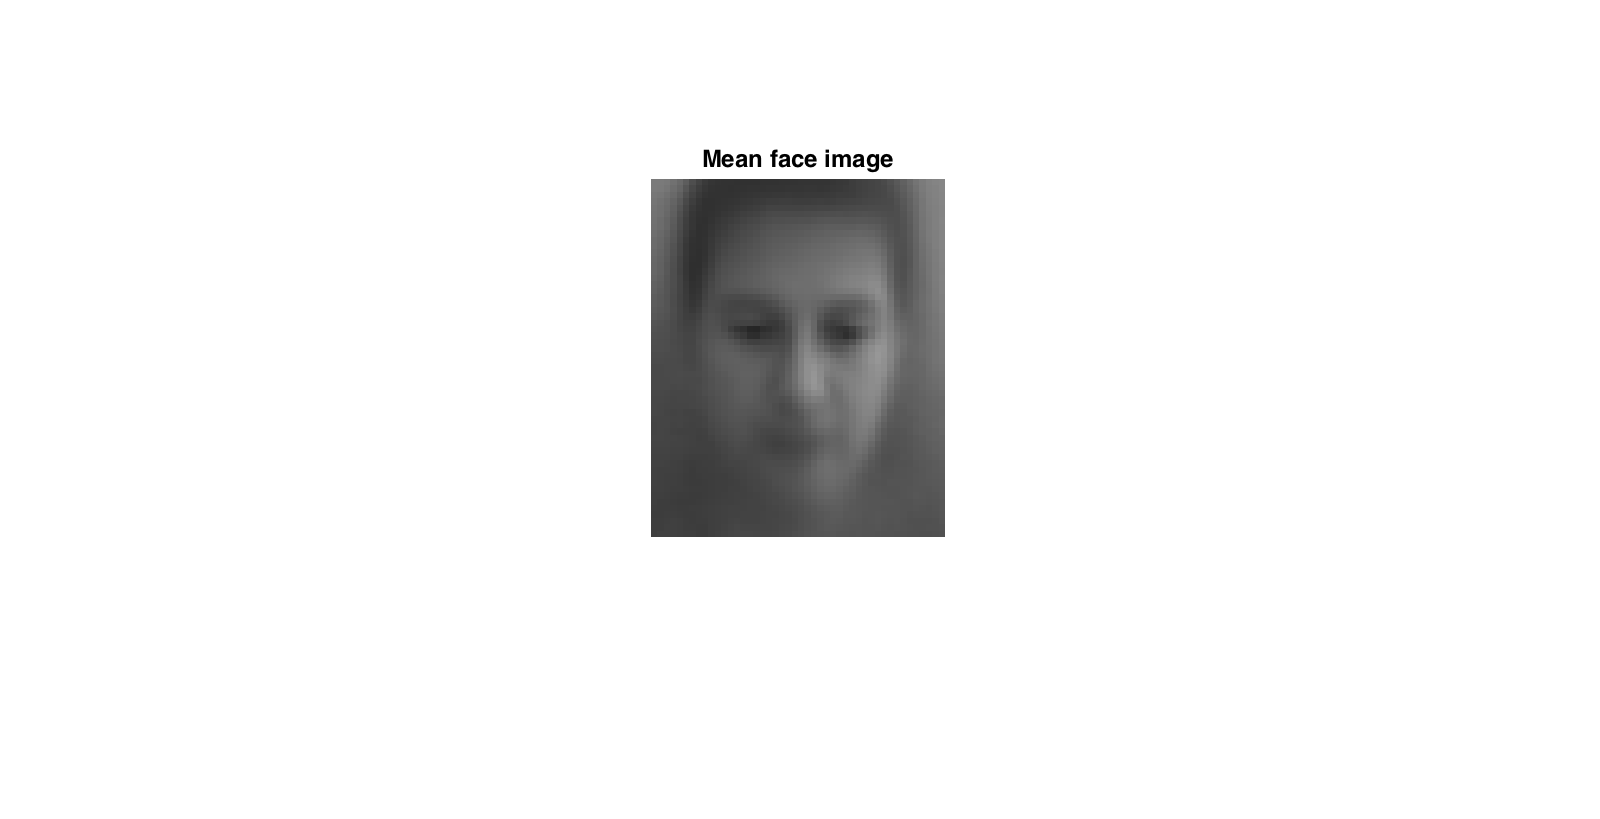
\includegraphics[width=0.8\linewidth]{q1_meanface}
		\caption{Mean face}
	\end{center}
	\label{fig:q1_meanface}
\end{figure}


Then, the all training faces were normalized by subtracting the mean face

\begin{equation}
\boldsymbol{\phi}_n = \boldsymbol{x_n} - \boldsymbol{\bar{x}}
\label{eq:q1_phi}
\end{equation}

and the matrix $\boldsymbol{A}$ can be acquired by

\begin{equation}
\boldsymbol{A} = [\phi_1, \phi_2, ..., \phi_N]
\label{eq:q1_A}
\end{equation}

Then the covariance matrix was calculated by

\begin{equation}
	\boldsymbol{S} = \frac{1}{N} A A^T
	\label{eq:q1_S}
\end{equation}

The eigenvectors $\boldsymbol{u_i}$ were calculated from the covariance matrix $S$ by $\boldsymbol{S u_i} = \lambda_i \boldsymbol{u_i}$. The dimension of the training data vector $x_n$ is $D = 2576$, denoted by $x_n \in R^D$ (for the data provided for this coursework). To reduce the dimension and maximising the variance of projected data, we selected M of the eigenvectors corresponding to the M largest eigenvalues $\lambda_i$ as eigenfaces. We found that among all the $\lambda_i$ ($i = 1,2, ..., D$), 415 out D eigenvalues were considered large (or non-zero), with order of magnitude ranging from 1 to 5. The remaining $D - 415 = 2161$ of the eigenvalues were considered as zeros with order of magnitude ranging from -10 to -13. In this coursework, we selected the largest $M = 50$ eigenfaces as the basis vectors for the face space. In Figure~\ref{fig:eigFaces}, we visualised 16 out of these 50 eigenfaces. The eigenfaces were visualised by reshaping the $x_n$ vector to a $56 \times 46$ matrix.

\begin{figure}
	\begin{center}
		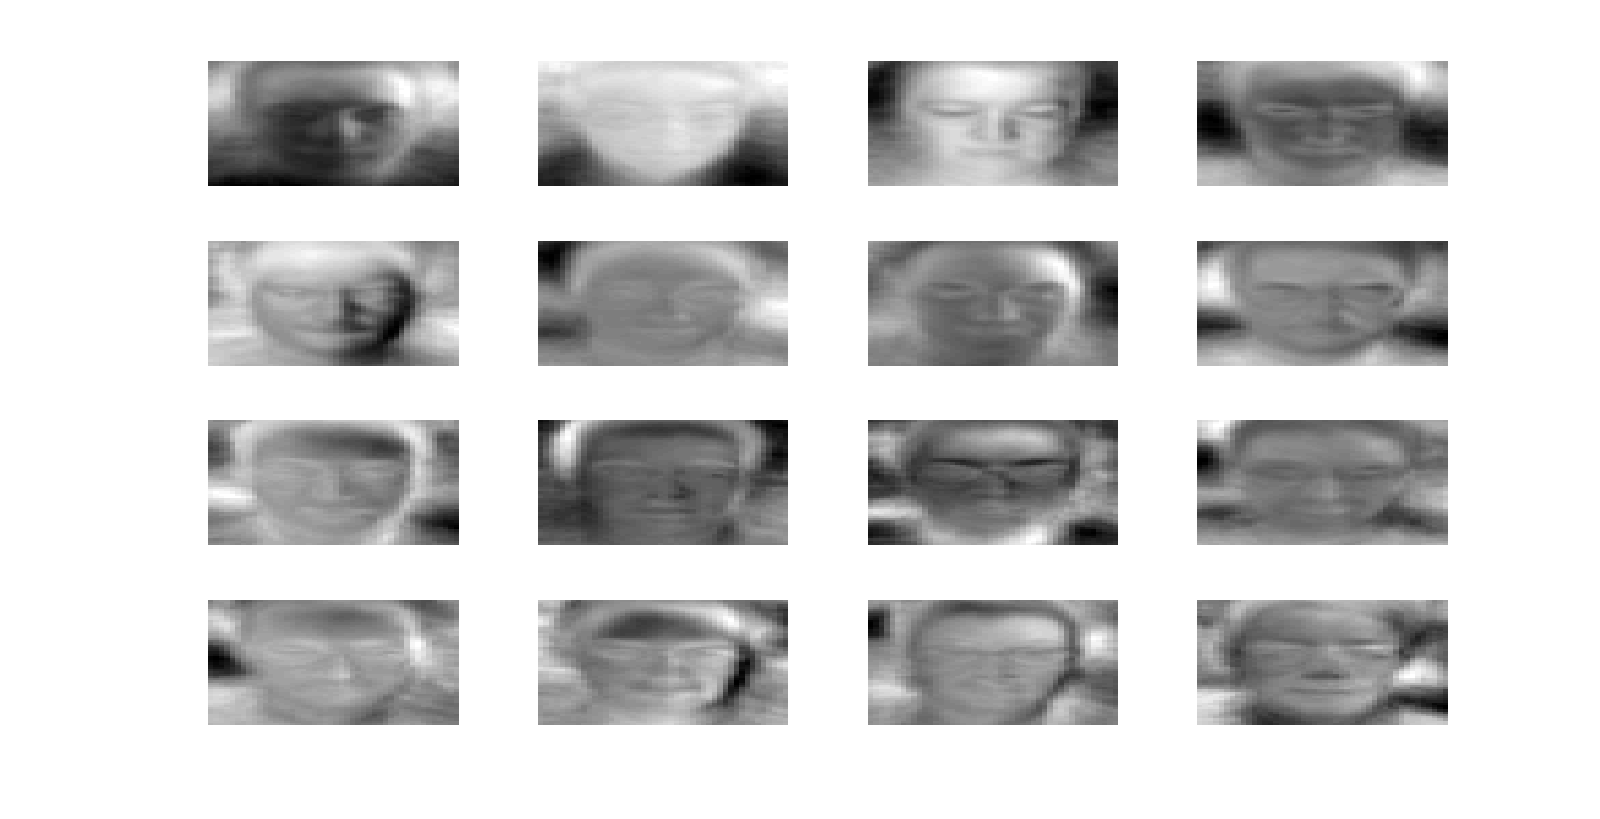
\includegraphics[width=0.8\linewidth]{q1_eigenfaces}
		\caption{The first 16 eigenfaces visualised}
		\label{fig:eigFaces}
	\end{center}
\end{figure}

To apply the PCA method, we projected every normalised training face $\phi_n$ to the M-dimensional subspace. Namely,
\begin{equation}
\omega_n = [a_{n1}, a_{n2}, ..., a_{nM}]
\label{eq:project}
\end{equation}

where the projection of $n$th image on the $i$th eigenface is denoted by

\begin{equation}
a_{ni} = \phi_n^T \boldsymbol{u_i}, ~  i = 1,...,M
\label{eq:project_a}
\end{equation}


Thus, the training faces were represented by its projections $\omega_n$. \\


\section{Question 2}
In this question, we discuss two different methods of calculating covariance matrix $S$ in the scope of PCA. It can be noticed from Eq.\ref{eq:q1_S} that the dimension of the covariance matrix is $D\times D$, which equals to the number of pixels in an image and is typically large. Under the consideration of computational efficiency, we implemented another proposed method, in which the covariance matrix is calculated by

\begin{equation}
S = \frac{1}{N} A^T A
\label{eq:S_q2}
\end{equation}

Since $A \in R^{D \times N}$, the covariance matrix now has dimension of $N \times N$, where $N$ equals to the number of images and is typically much smaller than $D$. As computing eigenvectors of large matrices is computational expensive, this method is preferred if proved equally effective for PCA. The resulting none-zero eigenvalues from Eq.\ref{eq:S_q2} had the same value of that using Eq.\ref{eq:q1_S}. The number of non-zero eigenvalues in this case is also 415. Note that the eigenvectors using this method were converted to the D-dimensional eigenvectors by 

\begin{equation}
	\boldsymbol{u_i} = A \boldsymbol{v_i}
\end{equation}

where $v_i$ denotes the eigenvectors calculated using the covariance matrix in Eq.\ref{eq:S_q2}. Figure~\ref{fig:q2_eigFaces} shows the visualised 16 eigenfaces. Comparing to the eigenfaces produced by the previous method (Figure~\ref{fig:eigFaces}), we notice that the face contour of the eigenfaces are the same. The difference in grey scale value could be caused by the randomisation of the data set and automatic normalisation by the image display function \texttt{imagesc} in MATLAB.\\

In conclusion, the methods for the computation of covariance matrix in Q1 and Q2 were proven equally effective for PCA, while the latter method is less computational expensive. Hence we used $S = (1/N) A^T A$ to compute the covariance matrix for image recognition in later sections of this coursework.


\begin{figure}
	\begin{center}
		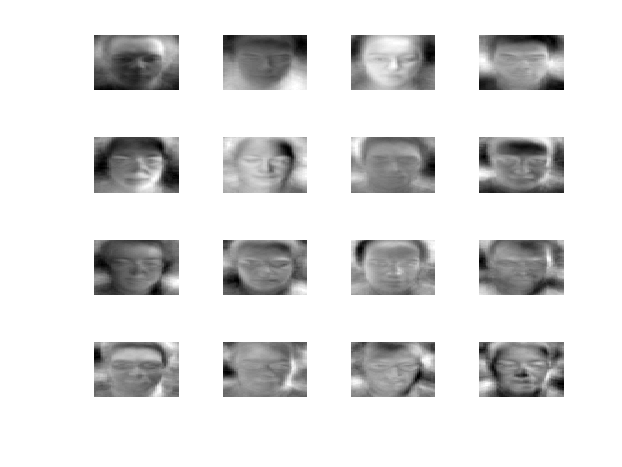
\includegraphics[width=1\linewidth]{q2_eigenfaces}
		\caption{The first 16 eigenfaces visualised for question 2}
		\label{fig:q2_eigFaces}
	\end{center}
\end{figure}

%\begin{figure*}
%\begin{center}
%\fbox{\rule{0pt}{2in} \rule{.9\linewidth}{0pt}}
%\end{center}
 %  \caption{Example of a short caption, which should be centered.}
%\label{fig:short}
%\end{figure*}

%------------------------------------------------------------------------
\section{Question 3}
The face images can be reconstructed from their projection on the M-dimensional subspace $\omega_n$ by

\begin{equation}
	\boldsymbol{\widetilde{x_n}} = \boldsymbol{\bar{x}} + \sum_{i=1}^M a_{ni} \boldsymbol{u_i}
	\label{eq:recon}
\end{equation}

where $\boldsymbol{\widetilde{x_n}}$ is the reconstructed face image. The reconstruction error, denoted as $J$ can be evaluated by

\begin{equation}
 J = \frac{1}{N} \sum_{n=1}^N || \boldsymbol{x_n} - \boldsymbol{\widetilde{x_n}}||^2
 \label{eq:J}
\end{equation}

where N is the total number of images. The formulation of PCA that we applied in this coursework maximises the variance of the projection of training data by spanning the face space using M eigenvectors $\{ \boldsymbol{u_i} \}$ of $S$ corresponding to the largest M eigenvalues $\{ \lambda_i \}$ where ($i = 1,2,...,M$). This formulation equivalently minimises the reconstruction error $J$ so it theoretically becomes

\begin{equation}
J_{theo} = \sum_{i=M+1}^{D^*} \lambda_i
\label{eq:J_theo}
\end{equation}

The $D^*$ in Eq.\ref{eq:J_theo} is the total number of eigenvectors of $S$. For the method we selected in Question 2, $D^* = 416$, which equals to the total number of training images. We evaluated and compared the experimental $J$ calculated by Eq. \ref{eq:J} and theoretical $J_{theo}$ calculated by Eq.\ref{eq:J_theo} while varying the number of M. Figure~\ref{fig:q3_J} presents $J$ and $J_{theo}$ as M varying from 40 to 100.\\
	
	\begin{figure}
		\begin{center}
			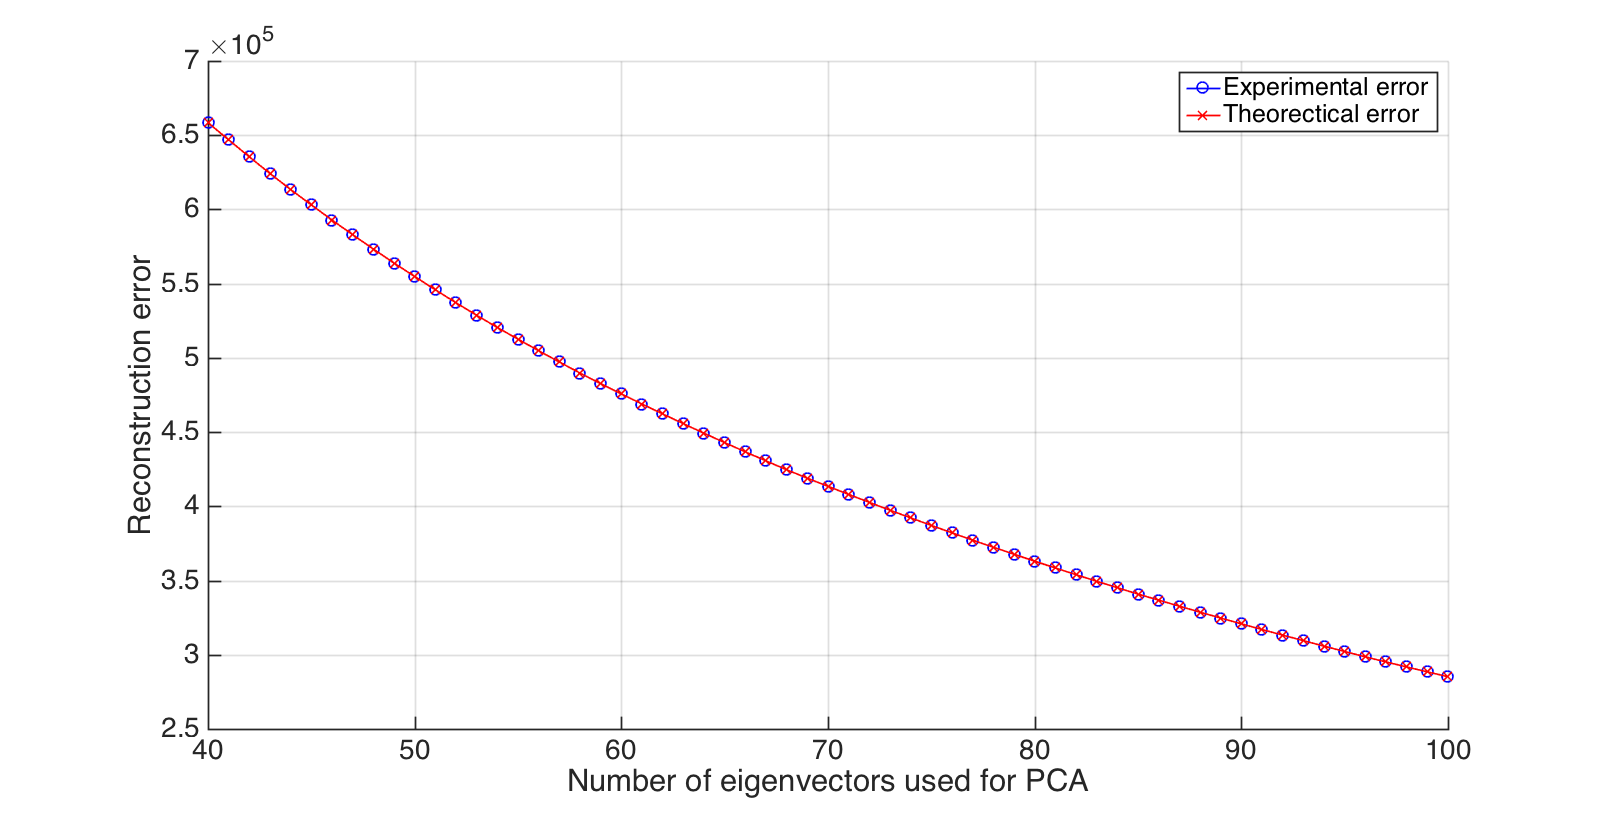
\includegraphics[width=1\linewidth]{q3_J}
			\caption{Reconstruction error, experimental vs theoretical}
			\label{fig:q3_J}
		\end{center}
	\end{figure}

It can be noticed that 1) the theoretical and experimental reconstruction errors are identical for all value of M; 2) the reconstruction error reduces when the number of M increases, but the gradient of the decreasing error curve reduces. This indicates that the positive effect of using more number of eigenfaces on reducing $J$ decreases as M increases. 

Figure~\ref{fig:q3_rec_train} shows the original training faces and the corresponding reconstructed images. Similarly, Figure~\ref{fig:q3_rec_test} shows the original testing faces and corresponding reconstructed images. As we can observe, the face images were well-reconstructed for both training and testing faces.
	
	\begin{figure}
		\begin{center}
			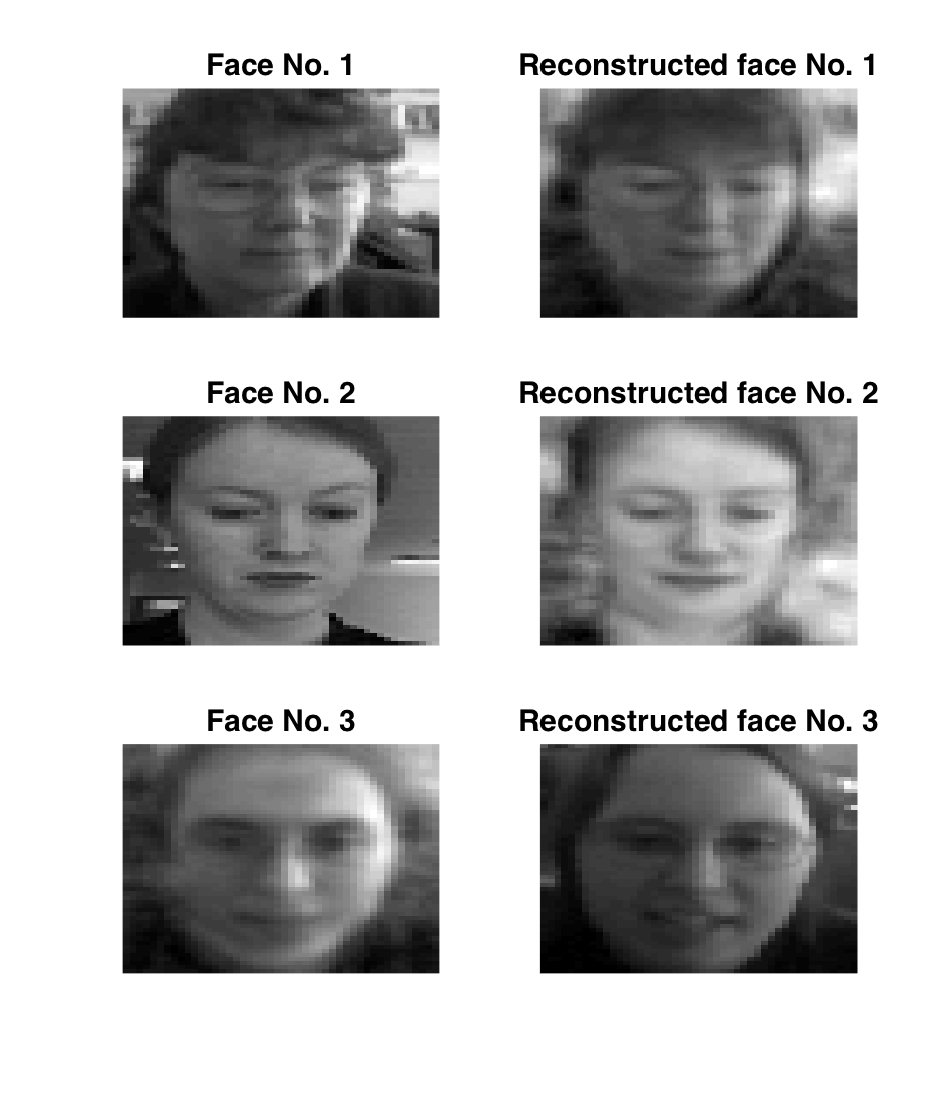
\includegraphics[width=1\linewidth]{q3_rec_train}
			\caption{Visualise reconstructed training images}
			\label{fig:q3_rec_train}
		\end{center}
	\end{figure}
	
	
	\begin{figure}
		\begin{center}
			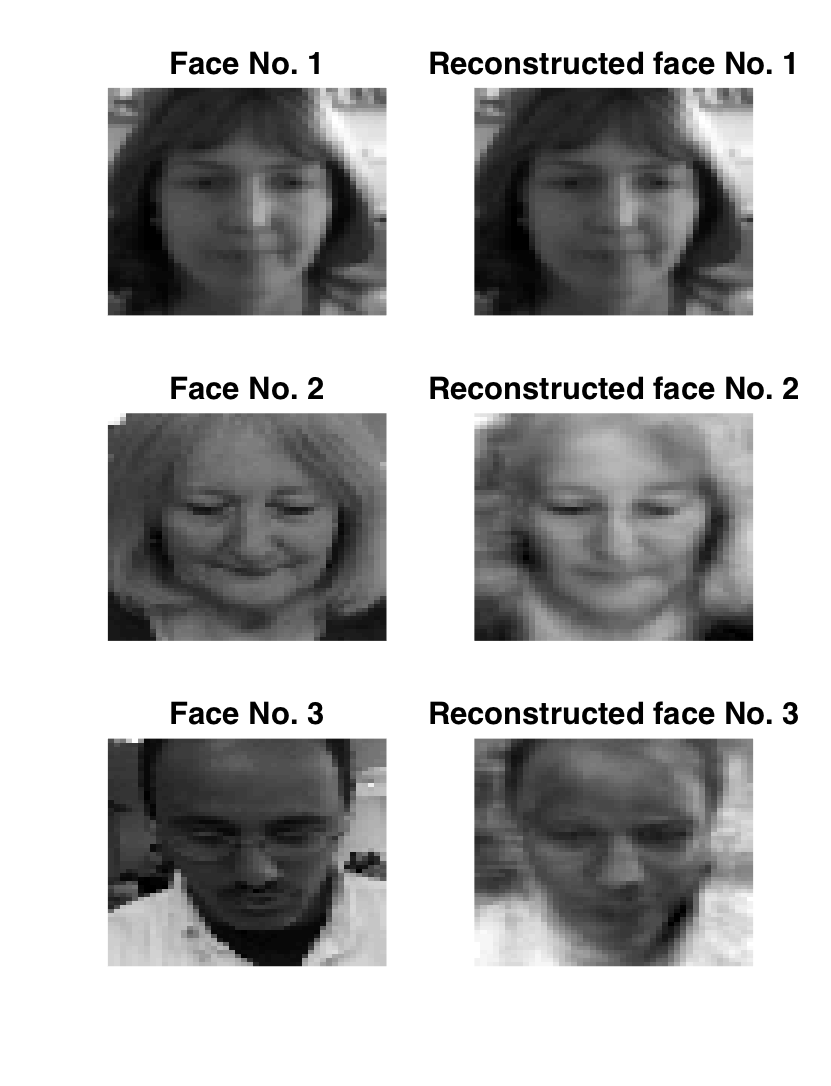
\includegraphics[width=1\linewidth]{q3_rec_test}
			\caption{Visualise reconstructed testing images}
			\label{fig:q3_rec_test}
		\end{center}
	\end{figure}

\section{Question 4}
At the training stage, the training images were projected on the M-dimensional face space. The $n^{th}$ image in the training set was represented  as $\omega_n$. At testing stage, each testing image was normalised by Eq.\ref{eq:q1_phi} and then projected on the eigenspace by Eq.\ref{eq:project_a} and represented as

$$ \omega = [a_1, a_2, ..., a_M]^T$$

This process transformed the testing images to represented data points that can be classified to a specific image in training set, thus effectively, recognised. In this coursework, the classification was achieved by Nearest Neighbour method and Alternative method. We shall now discuss and compare the two methods.

\subsection{Nearest Neighbour classification}
In the Nearest Neighbour (NN) classification, the testing image is assigned to the class which has the minimum error $e$, which is calculated with respect to all training images as

\begin{equation}
	e = || \omega - \omega_n||, ~ n = 1, ..., N
\end{equation}
where recall N is the number of training images. 

\subsubsection{Accuracy of recognition}
Each of the testing image was assigned a label indicating which class the image was classified to. This is referred to as prediction in the report. To evaluate the accuracy of recognition, we calculated correction rate by 

\begin{equation}
	correction~ rate = \frac{number~of~correct~prediction}{number~of ~testing~image}
	\label{eq:R_correct}
\end{equation}

The correction rate of PCA based face recognition can be affected by the number of eigenvector used to span the face subspace $M$. Hence, we varied the number of $M$ from 1 to 100 and calculated the corresponding correction rate. Considering the randomness of data partition, we iterated the traing-testing process for 50 times for each value of $M$ and averaged the correction rate. The result of the calculations are presented in Figure~\ref{fig:q4_nn_rate}. The correction rate increased rapidly as $M$ increased from 1 to around 30 and then converged to approximately 65\%. This indicates that it is unnecessary to use large number of eigenvector basis $\boldsymbol{u_i}$, despite there are 415 of $\boldsymbol{u_i}$ corresponding to largest eigenvalues available. As the computational complexity increases when $M$ increases, we came to the conclusion that a optimal value of $M$ is around 50-60 for this particular situation, as the correction rate started to converge in this region. 


	\begin{figure}
		\begin{center}
			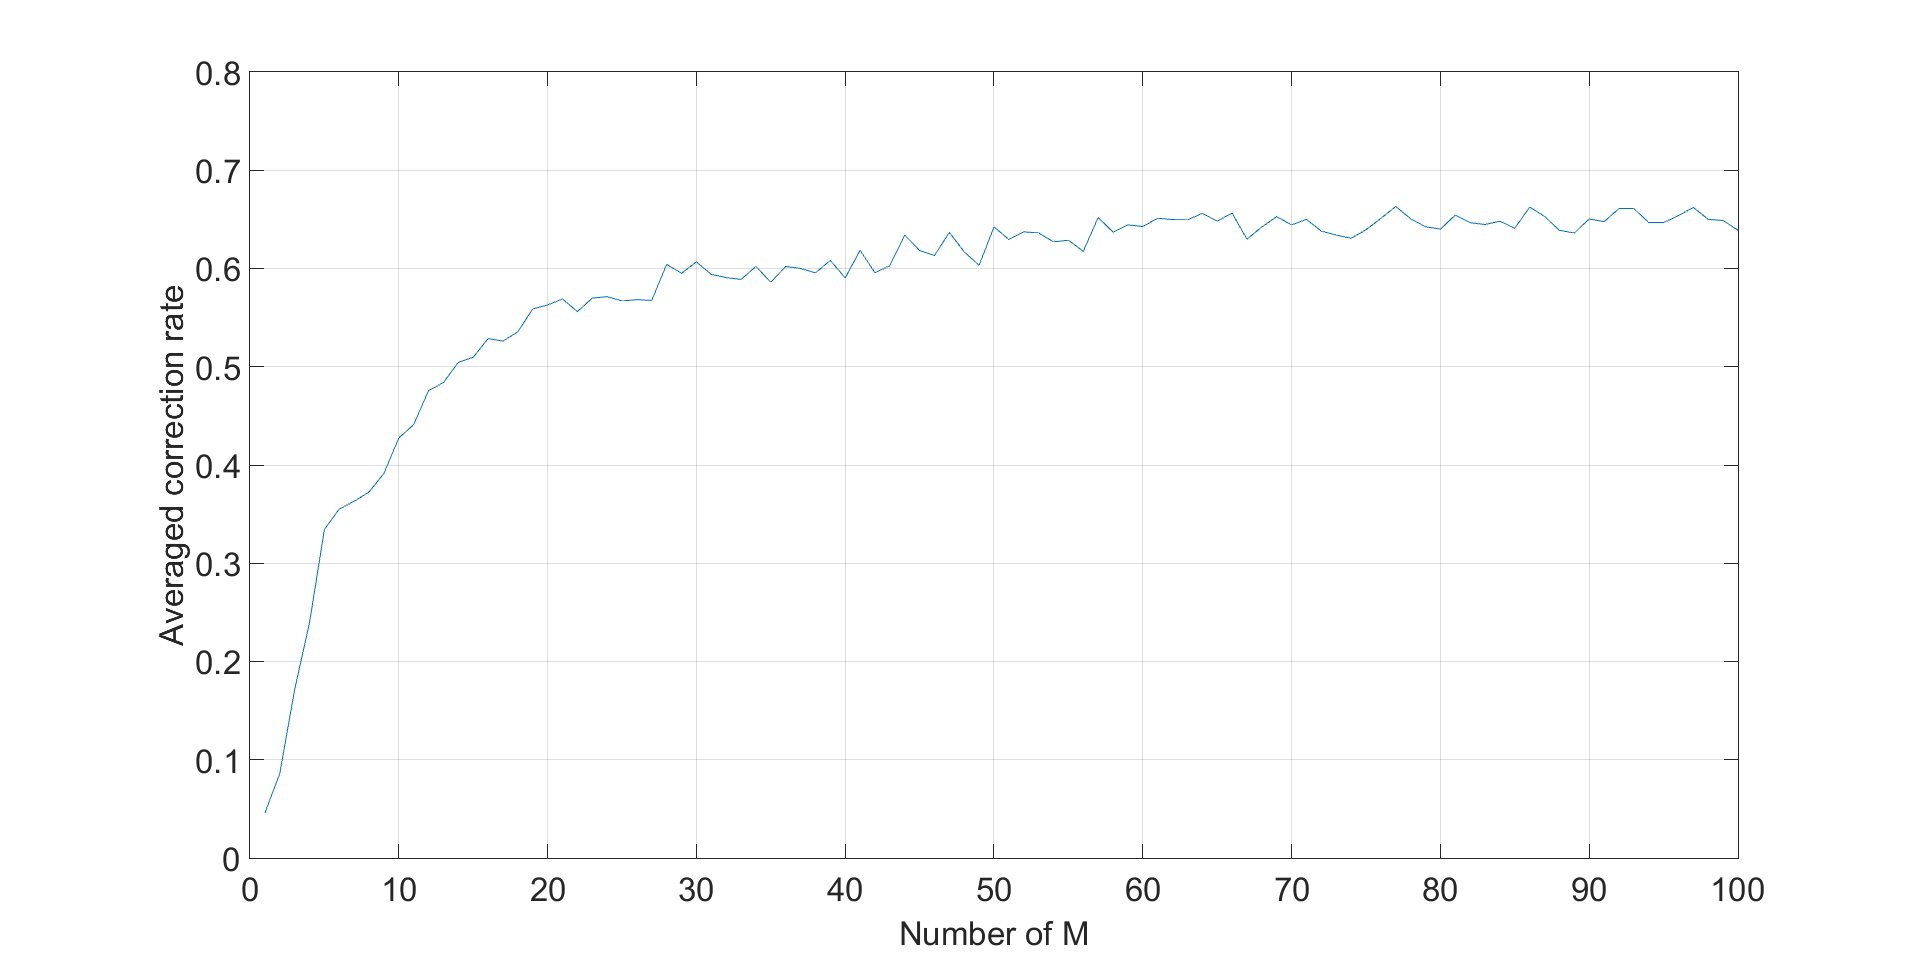
\includegraphics[width=1\linewidth]{correctRate_NN}
			\caption{Correction rate of NN method}
			\label{fig:q4_nn_rate}
		\end{center}
	\end{figure}
	
	
\subsubsection{Example of failure cases}
We now discuss the cases of failure for NN method classification. Two examples of failed classifications are shown in image (a) and (c) in Figure~\ref{fig:q4_nn_fail}. In this figure, image (b) and (d) are the images from the classes that image (a) and (c) were classified to in testing. In both comparison between both pairs (a)-(b) and (c)-(d), we can observe some non-decisive similarities in terms of facial feature. Similar comparisons were made on other misclassified testing images. However, no clear visual indication of the cause of incorrect recognition was established.

	\begin{figure}
		\begin{center}
			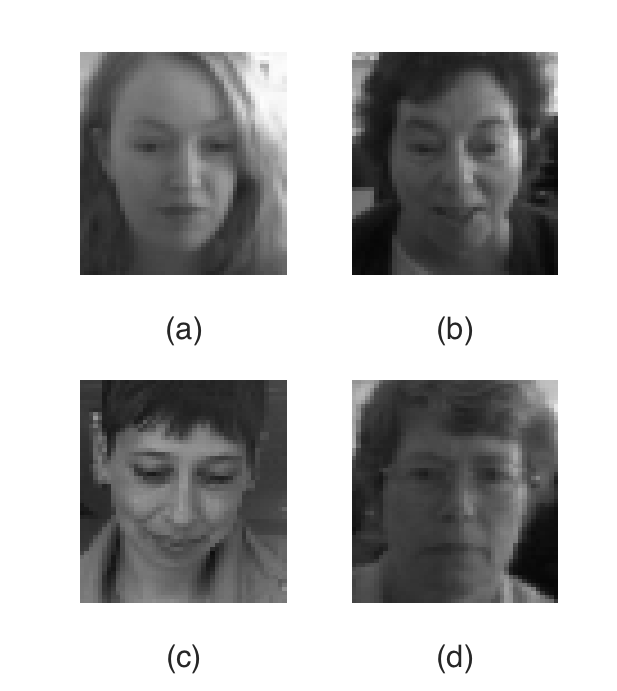
\includegraphics[width=0.9\linewidth, height = 6cm]{q4_fail_NN}
			\caption{(a)\&(c) Image of failed cases for NN method;  (b)\&(d) sample image from the class (a)\&(c) are classified as}
			\label{fig:q4_nn_fail}
		\end{center}
	\end{figure}

\subsubsection{Confusion matrix}
The confusion matrix provides a visual impression of the recognition result. The confusion matrix of PCA based face recognition using NN classification is presented in Figure~\ref{fig:q4_confmat_nn}, which corresponds to a correction rate of 63\%. In the confusion matrix, the colour patches on the diagonal indicate correct predictions. Correspondingly, patches appeared on places other than the diagonal indicate a case of incorrect classification and the number of misclassified cases are indicated by the colour. 

	\begin{figure}
		\begin{center}
			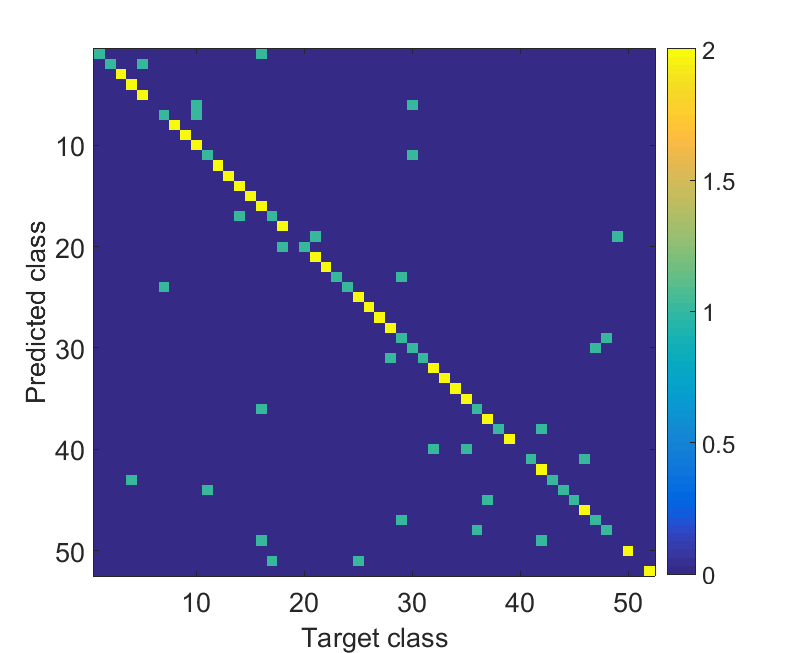
\includegraphics[width=0.9\linewidth, height = 6cm]{confusion_matrix_NN}
			\caption{Confusion matrix of NN classification, $M = 100$}
			\label{fig:q4_confmat_nn}
		\end{center}
	\end{figure}


\subsection{Alternative method for classification}
An alternative method oppose to the NN method was implemented in our coursework for classification of data points $\omega$. This method computes the eigenvectors and creates face subspace for every class separately and store the subspaces as training knowledge. At testing stage, the testing image was projected to individual subspaces using the Eq.\ref{eq:project_a} and reconstructed using Eq.\ref{eq:recon}. The assignment of predicted label depends on the measurement of reconstruction error by

\begin{equation}
	\hat{y} = arg_i ~ min || \boldsymbol{x} - \boldsymbol{\widetilde{x_i}}||
\end{equation}

where $\boldsymbol{x}$ is the testing image and $\boldsymbol{\widetilde{x_i}}$ is the reconstructed testing image using the eigenvector subspace computed from the $i$th class.

\subsubsection{Accuracy of recognition}
We tested all available testing images and calculate the correction rate as a measure of recognition accuracy. The correction rate is calculated using the same method used in NN method (Eq.\ref{eq:R_correct}). Similarly, we varied the number of eigenvectors used in each class to span the face subspace for the classes. Thus the number of eigenvector basis $M_{alter}$ can be varied between 1 and 8 and the total number of eigenvectors used is $52 \cdot M_{alter}$. Figure~\ref{fig:q4_alter_rate} is the resulting correction rate plotted against the value of $M_{alter}$. Same as in NN method, the correction rate was averaged over 50 iterations for every value of $M_{alter}$. The result indicates that 1) the alternative method achieved better correction rate than the NN method; 2) the conclusion regarding the impact of number of eigenvector used to the accuracy drawn from the result of the NN method is also valid. 


	\begin{figure}
		\begin{center}
			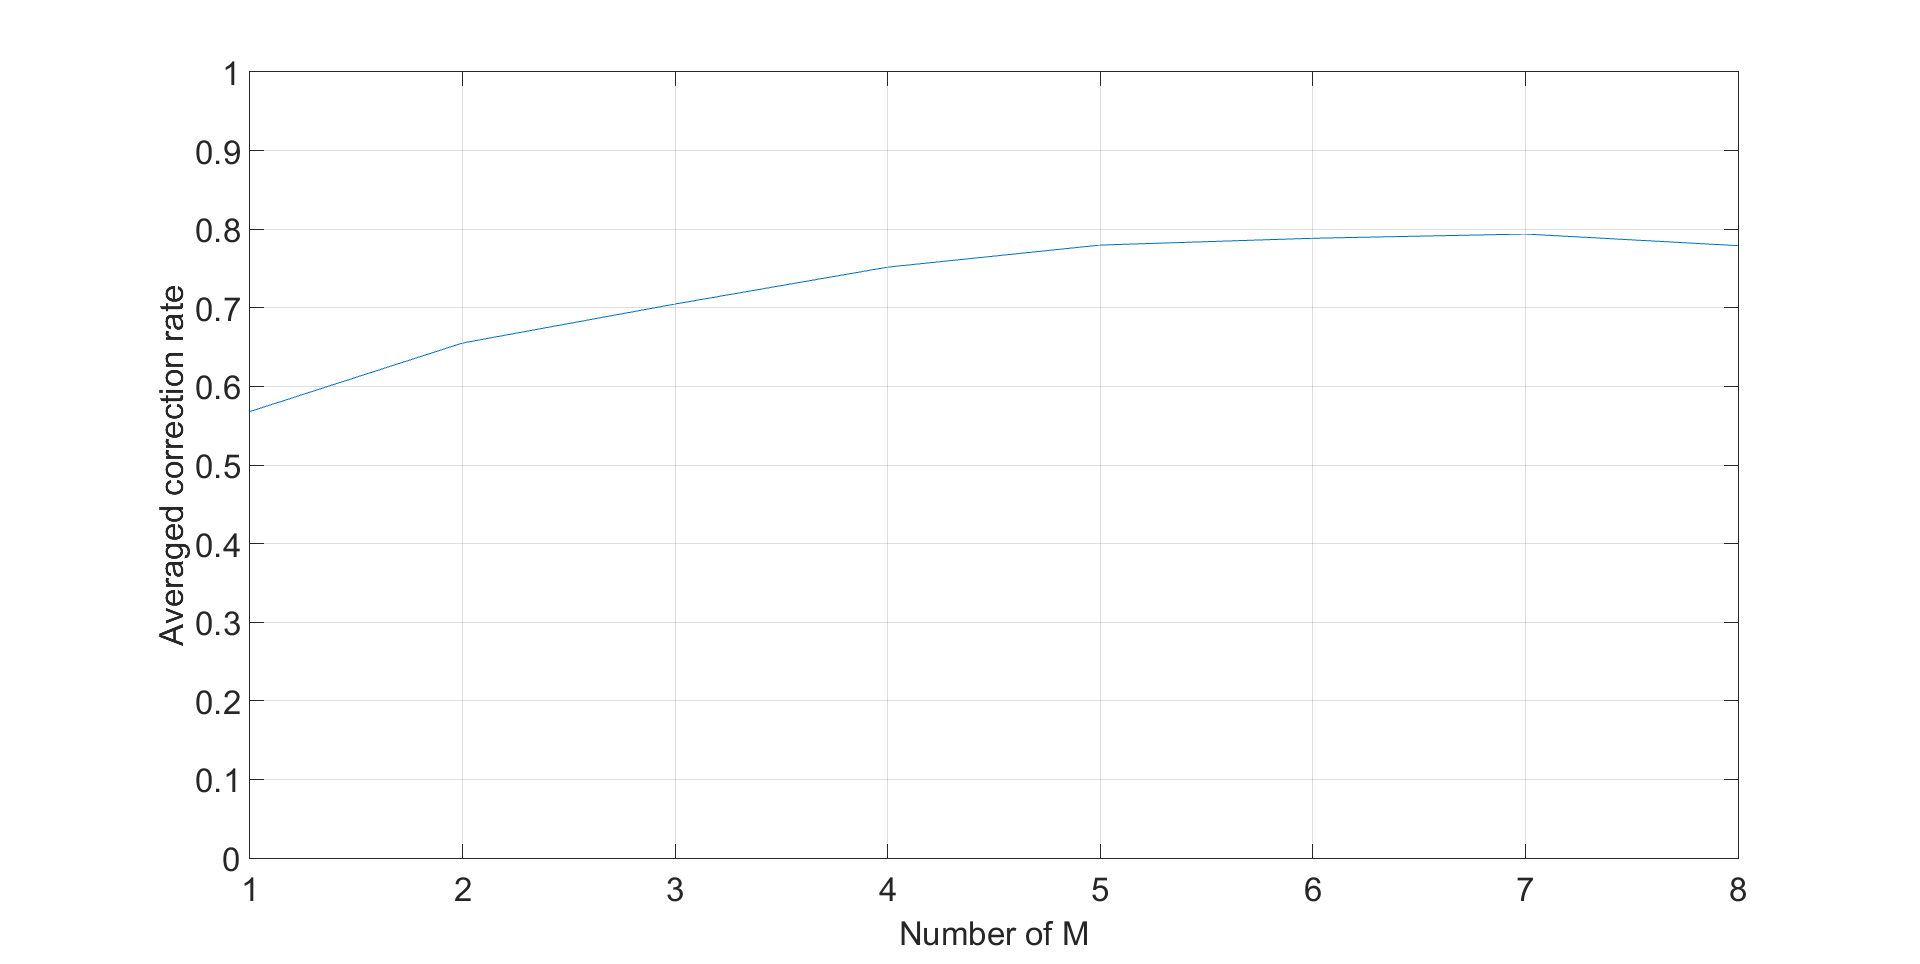
\includegraphics[width=0.9\linewidth]{correctRate_alter}
			\caption{Correction rate for the alternative method}
			\label{fig:q4_alter_rate}
		\end{center}
	\end{figure}


\subsubsection{Example of failure cases}
Here in Figure~\ref{fig:q4_alter_fail}, we demonstrate the cases of failed recognition as in NN method to visually exam the misclassification. Again we can observe some suspicious cause of misclassification such as the similarity of lighting in between (a) and (b), or the similarity of the shape of forehead between (c) and (d). However, these observations are rather intuitive and subjective and thus cannot be related to the condition that caused misclassification. The fact that the significant features (i.e. eigenfaces) extracted for PCA based recognition are not necessarily related with typical visual features (e.g. eyes, nose, mouth etc.), visual examination of failure cases may not be a constructive effort to identify the cause of failure.

	\begin{figure}
		\begin{center}
			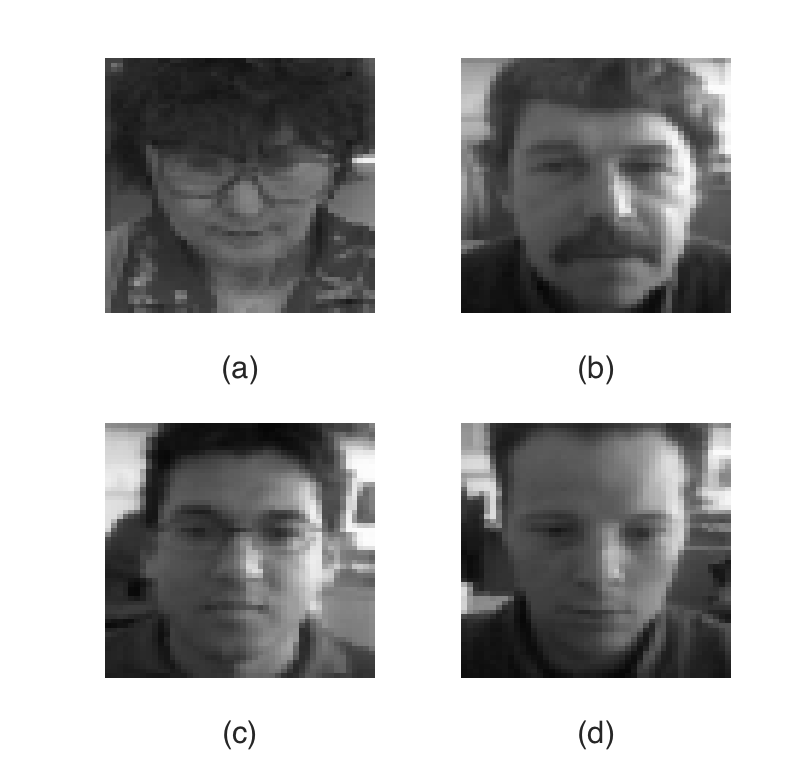
\includegraphics[width=0.9\linewidth]{q4_fail_alter}
			\caption{Failed cases for the alternative method}
			\label{fig:q4_alter_fail}
		\end{center}
	\end{figure}

\subsubsection{Confusion matrix}
Figure~\ref{fig:q4_confmat_alter} show the confusion matrix of alternative method of classification, which corresponds to a correction rate of 78\%. \\

	\begin{figure}
		\begin{center}
			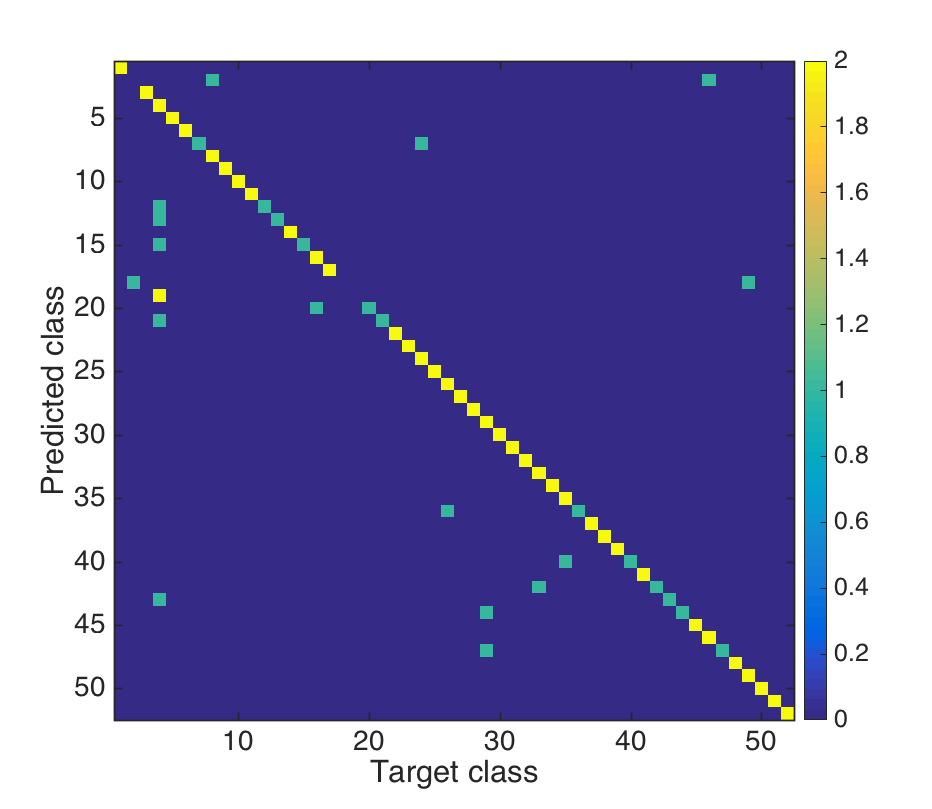
\includegraphics[width=0.9\linewidth]{confusion_matrix_alter}
			\caption{Confusion matrix of alternative method classification, $M_{alter} = 8$}
			\label{fig:q4_confmat_alter}
		\end{center}
	\end{figure}

\subsection{Comparison between NN and alternative method}
\begin{enumerate}
	\item Accuracy\\
	As we can see from Figure~\ref{fig:q4_nn_rate} and ~\ref{fig:q4_alter_rate}, the alternative method achieved higher accuracy in general. However, it's worth mentioning that the minimum amount of eigenvectors required for the alternative method is 52 (i.e. $M_{alter} = 1$). The accuracy rate achieved at this number of $M_{alter}$ is lower than the accuracy of NN method with ($M = 52$). Other than this exception, the alternative method delivered better recognition accuracy.\\
	
	\item Time consumption\\
	To compare the two classification methods in terms of time efficiency, we measured the time consumed by the training and testing program by the stopwatch in MATLAB \texttt{tic} and \texttt{toc}. Again, we varied the number of eigenvectors used to measure the effect of that too. Figure~\ref{fig:q4_time_nn} and ~\ref{fig:q4_time_alter} show the training time, testing time and total time of NN method and the alternative method respectively. It can be concluded from the results that: a) the training time contributed to the majority of total time consumption for both methods; b) the time required for the NN method did not increase with increasing number of $M$, while the training time of the alternative method had a noticeable increase. This conclusion in particular reveals a trade-off between time consumption and accuracy for the alternative method when selecting the value of $M_{alter}$; c) the alternative method are more time consuming than the NN method. 
	
	\begin{figure}
		\begin{center}
			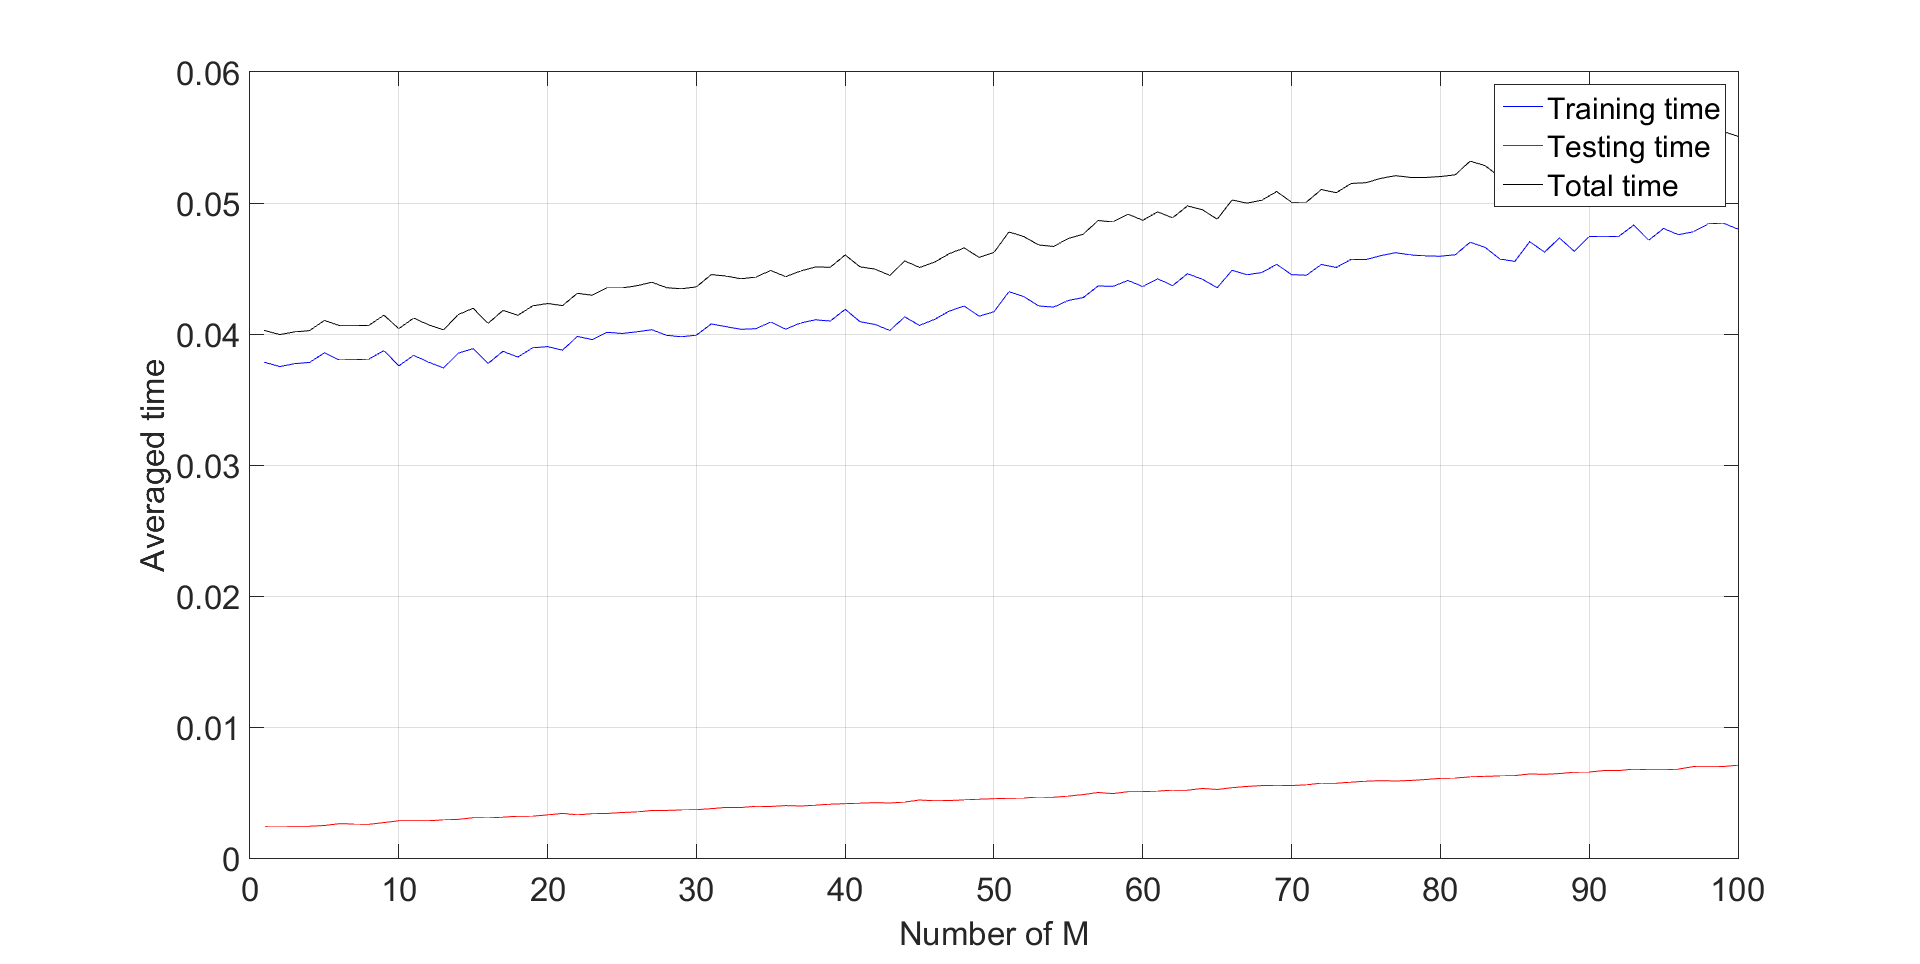
\includegraphics[width=0.9\linewidth]{time_NN}
			\caption{Time consumed for the NN method}
			\label{fig:q4_time_nn}
		\end{center}
	\end{figure}
	
		\begin{figure}
			\begin{center}
				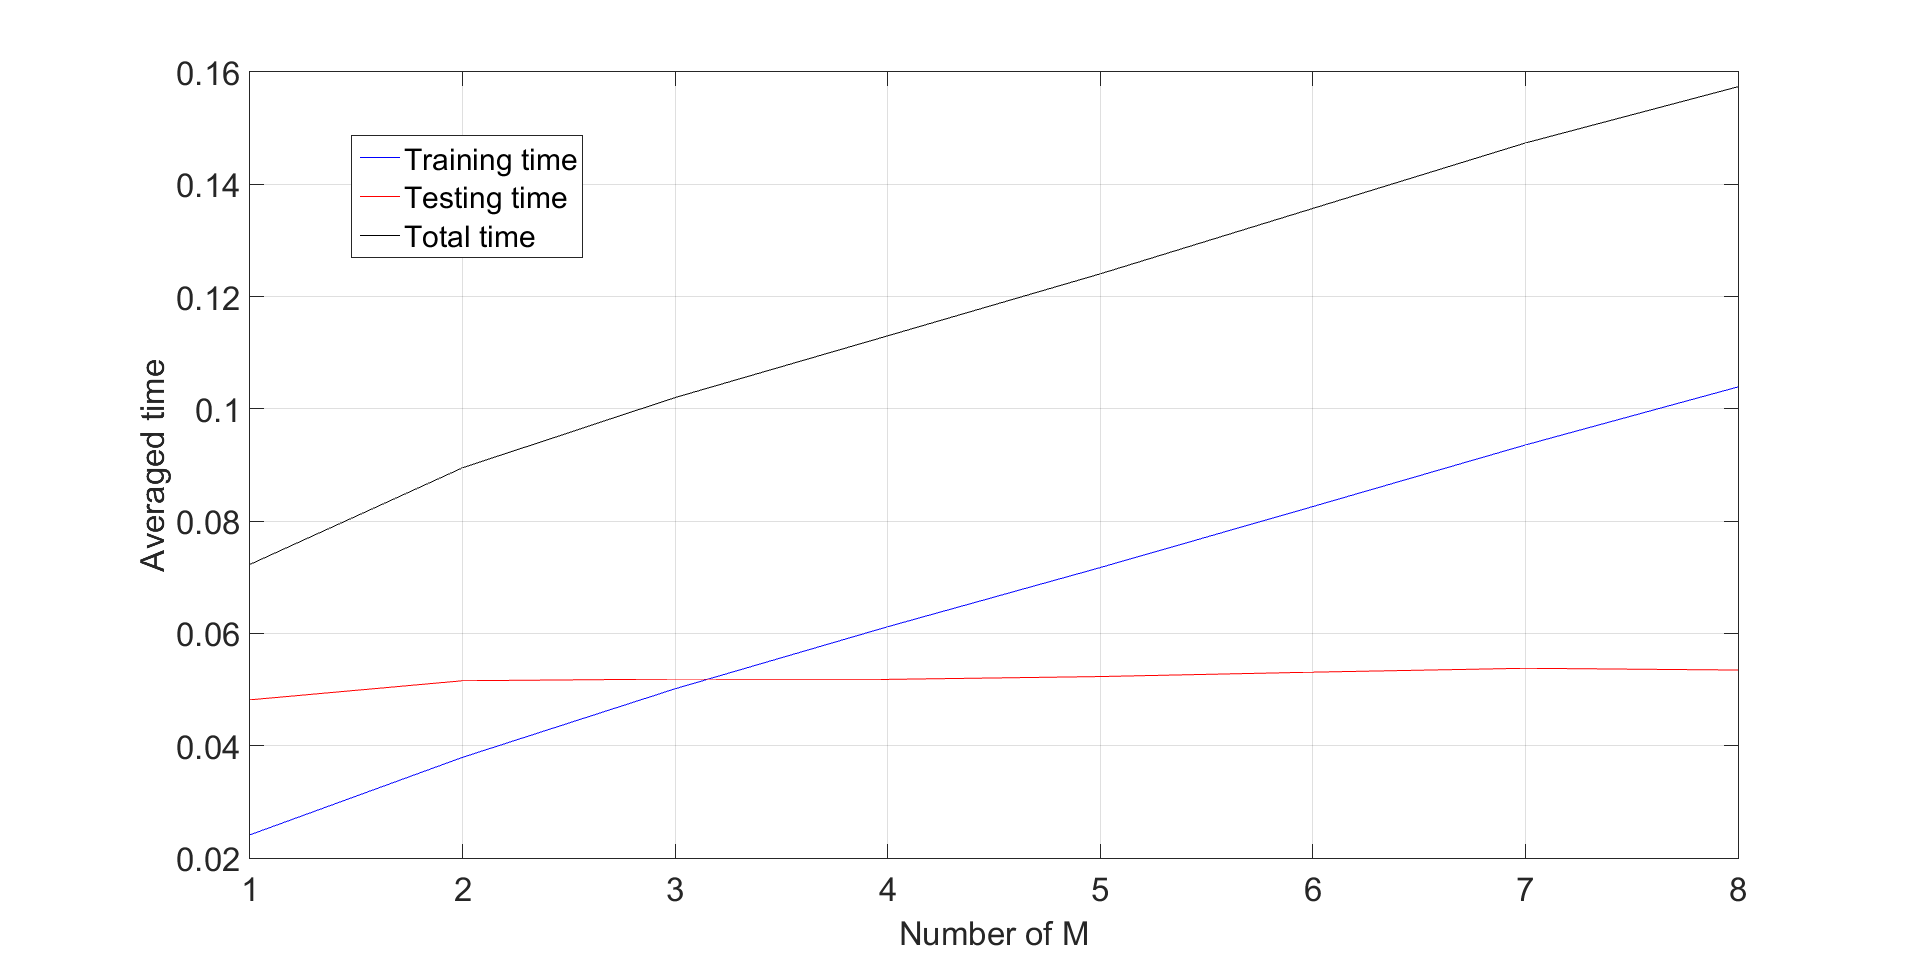
\includegraphics[width=0.9\linewidth]{time_alter}
				\caption{Time consumed for the alternative method}
				\label{fig:q4_time_alter}
			\end{center}
		\end{figure}
	
	\item Memory \\
	If we assume that the same amount of eigenvectors ($M$) were used for both methods, it can be found that both the NN method and the alternative method requires to store data of size $[M \times D]$ ($M = M_{alter} \times 52$ for the alternative method). Consequentially, the memory requirement of the two classification methods is primarily affected by the number and size of eigenvectors, as they are also most memory demanding and cannot be released during both training and testing period. However, it can be observed from Figure~\ref{fig:q4_nn_rate} and ~\ref{fig:q4_alter_rate}, the NN method requires fewer eigenvectors, equivalently fewer memory, to achieve its maximum accuracy.
	
\end{enumerate}

\cite{Kim16}

{\small
\bibliographystyle{ieee}
\bibliography{egbib}
}

%\onecolumn
%\appendix
%\section{Appendix 1 Matlab Code}
%\subsection{Init.m}
%\lstinputlisting{init.m}
%
%\section{matlab code part 2}
%\lstinputlisting{init.m}



\end{document}
